\documentclass[11pt,a4paper]{article}
\usepackage[utf8]{inputenc}
\usepackage[T1]{fontenc}
\usepackage[margin=2.5cm]{geometry}
\usepackage{amsmath,amssymb}
\usepackage{graphicx}
\usepackage{listings}
\usepackage{xcolor}
\usepackage{hyperref}
\usepackage{float}
\usepackage{booktabs}
\usepackage{caption}

% Code listing style
\definecolor{codebg}{RGB}{245,245,245}
\definecolor{codegreen}{RGB}{0,128,0}
\definecolor{codegray}{RGB}{128,128,128}
\definecolor{codeblue}{RGB}{0,0,180}
\lstdefinestyle{cstyle}{
    backgroundcolor=\color{codebg},
    basicstyle=\ttfamily\footnotesize,
    breaklines=true,
    captionpos=b,
    commentstyle=\color{codegreen},
    keywordstyle=\color{codeblue}\bfseries,
    stringstyle=\color{red},
    numberstyle=\tiny\color{codegray},
    numbers=left,
    numbersep=5pt,
    language=C,
    frame=single,
    tabsize=4,
    showstringspaces=false
}
\lstset{style=cstyle}

\title{\textbf{TP6: MPI Derived Types} \\ \large Parallelization Course Report}
\author{Student Report}
\date{March 3, 2026}

\begin{document}
\maketitle
\tableofcontents
\newpage

% ============================================================
\section{Introduction}

This report covers TP6 on \textbf{MPI Derived Types}. MPI derived datatypes allow users to describe non-contiguous memory layouts so that data can be sent and received in a single communication call, avoiding manual packing/unpacking. We implement two exercises:

\begin{enumerate}
    \item \textbf{Exercise 1}: Matrix transposition during communication using \texttt{MPI\_Type\_vector} and \texttt{MPI\_Type\_create\_hvector}.
    \item \textbf{Exercise 2}: Distributed batch gradient descent using \texttt{MPI\_Type\_create\_struct} to define a custom datatype for training samples.
\end{enumerate}

% ============================================================
\section{Exercise 1: Matrix Transposition using Derived Types}

\subsection{Problem Statement}

A matrix $A$ of size $4 \times 5$ is initialized on process~0 with values $1$ through $20$. The goal is to send $A$ from process~0 to process~1 such that process~1 receives the \textbf{transposed matrix} $A^T$ of size $5 \times 4$ directly in memory, using a single \texttt{MPI\_Send}/\texttt{MPI\_Recv} pair and MPI derived datatypes.

\subsection{Approach}

The key insight is that transposition corresponds to a specific reordering of memory. We construct a derived type on the receiver side that maps the incoming row-major data into column-major positions of the destination array.

\subsubsection{Step 1: Column Type (\texttt{MPI\_Type\_vector})}

We define a vector type that selects one ``column'' of the transposed matrix \texttt{at[5][4]}:

\begin{lstlisting}
MPI_Type_vector(COLS,        // count: 5 blocks
                1,           // blocklength: 1 element per block
                ROWS,        // stride: 4 elements apart
                MPI_DOUBLE,  // base type
                &column_type);
\end{lstlisting}

This selects elements \texttt{at[0][j]}, \texttt{at[1][j]}, \ldots, \texttt{at[4][j]} for a given column index $j$. The stride of \texttt{ROWS}~(4) skips over one full row of \texttt{at} between each selected element.

\subsubsection{Step 2: Full Transpose Type (\texttt{MPI\_Type\_create\_hvector})}

We replicate the column type \texttt{ROWS}~(4) times, each shifted by exactly \texttt{sizeof(double)} bytes:

\begin{lstlisting}
MPI_Type_create_hvector(ROWS,              // count: 4 columns
                        1,                 // blocklength: 1 column_type
                        sizeof(double),    // stride in bytes
                        column_type,       // base type
                        &transpose_type);
\end{lstlisting}

The byte-level stride of \texttt{sizeof(double)} moves to the next column of \texttt{at} (i.e., one element to the right within each row).

\subsubsection{Communication}

\begin{itemize}
    \item \textbf{Process 0}: sends the matrix as a contiguous block of $4 \times 5 = 20$ doubles.
    \item \textbf{Process 1}: receives using the committed \texttt{transpose\_type}, which places data in transposed order.
\end{itemize}

\subsection{Memory Layout Illustration}

\begin{verbatim}
Source (process 0) row-major:
 [ 1  2  3  4  5 | 6  7  8  9 10 | 11 12 13 14 15 | 16 17 18 19 20]
   row 0           row 1           row 2             row 3

Destination (process 1) at[5][4] after transposition:
 [  1  6 11 16 ]   row 0 of A^T  (= column 0 of A)
 [  2  7 12 17 ]   row 1 of A^T  (= column 1 of A)
 [  3  8 13 18 ]   row 2
 [  4  9 14 19 ]   row 3
 [  5 10 15 20 ]   row 4
\end{verbatim}

\subsection{Source Code}

\lstinputlisting[caption={ex1\_transpose.c --- Matrix Transposition with MPI Derived Types}]{ex1_transpose.c}

\subsection{Expected Output}

\begin{verbatim}
Process 0 - Matrix a:
  1  2  3  4  5
  6  7  8  9 10
 11 12 13 14 15
 16 17 18 19 20
Process 1 - Matrix transposee at:
  1  6 11 16
  2  7 12 17
  3  8 13 18
  4  9 14 19
  5 10 15 20
\end{verbatim}

\subsection{Compilation and Execution}

\begin{verbatim}
mpicc -O2 -Wall -std=c99 -o ex1_transpose ex1_transpose.c
mpirun -np 2 ./ex1_transpose
\end{verbatim}

% ============================================================
\section{Exercise 2: Distributed Gradient Descent with MPI Derived Types}

\subsection{Problem Statement}

Implement a distributed batch gradient descent algorithm using MPI. Each training sample is a structure containing a feature vector \texttt{x[N\_FEATURES]} and a scalar label \texttt{y}. The struct is communicated using a custom MPI datatype defined with \texttt{MPI\_Type\_create\_struct}.

The model is a simple linear regression:
$$\hat{y} = \sum_{f=0}^{F-1} w_f \cdot x_f + w_F$$
where $w_F$ is the bias term. The loss function is Mean Squared Error (MSE):
$$\mathcal{L} = \frac{1}{N} \sum_{i=1}^{N} (\hat{y}_i - y_i)^2$$

\subsection{MPI Derived Type for Sample}

The \texttt{Sample} structure:
\begin{lstlisting}
typedef struct {
    double x[N_FEATURES];  // feature vector
    double y;              // label
} Sample;
\end{lstlisting}

The derived type is created with \texttt{MPI\_Type\_create\_struct}:

\begin{lstlisting}
int block_lengths[2] = {N_FEATURES, 1};
MPI_Aint displacements[2];
MPI_Datatype types[2] = {MPI_DOUBLE, MPI_DOUBLE};

// Compute byte displacements using MPI_Get_address
MPI_Get_address(&dummy,   &base_addr);
MPI_Get_address(&dummy.x, &x_addr);
MPI_Get_address(&dummy.y, &y_addr);
displacements[0] = x_addr - base_addr;
displacements[1] = y_addr - base_addr;

MPI_Type_create_struct(2, block_lengths, displacements, types, &sample_type);

// Resize to match actual struct size (handles compiler padding)
MPI_Type_create_resized(sample_type, 0, sizeof(Sample), &resized);
MPI_Type_commit(&resized);
\end{lstlisting}

The \texttt{MPI\_Type\_create\_resized} call is critical: it ensures the extent of the type matches \texttt{sizeof(Sample)}, which is necessary for correct behavior with \texttt{MPI\_Scatterv} on arrays of \texttt{Sample}.

\subsection{Algorithm}

\begin{enumerate}
    \item \textbf{Data generation}: Process~0 generates $N$ samples with the true model $y = 2x_0 - x_1 + 0.5 + \epsilon$.
    \item \textbf{Scatter}: The dataset is distributed using \texttt{MPI\_Scatterv} with the custom type.
    \item \textbf{Local computation}: Each process computes its local gradient and local MSE loss.
    \item \textbf{Global reduction}: \texttt{MPI\_Allreduce} aggregates gradients and losses.
    \item \textbf{Weight update}: All processes update weights identically: $w \leftarrow w - \eta \cdot \nabla\mathcal{L}$.
    \item \textbf{Early stopping}: Training stops when MSE $< 10^{-2}$.
\end{enumerate}

\subsection{Source Code}

\lstinputlisting[caption={distrib\_grad.c --- Distributed Gradient Descent}]{distrib_grad.c}

\subsection{Actual Output (4 processes, 1000 samples)}

\begin{verbatim}
Epoch   10 | Loss (MSE): 1.680855 | w[0]: 0.1326, w[1]: -0.0673, bias: 0.0825
Epoch   20 | Loss (MSE): 1.437848 | w[0]: 0.2566, w[1]: -0.1301, bias: 0.1505
Epoch   30 | Loss (MSE): 1.234764 | w[0]: 0.3725, w[1]: -0.1888, bias: 0.2066
...
Epoch  390 | Loss (MSE): 0.011282 | w[0]: 1.8670, w[1]: -0.9357, bias: 0.4948
Epoch  400 | Loss (MSE): 0.010261 | w[0]: 1.8761, w[1]: -0.9401, bias: 0.4952
Early stopping at epoch 403 -- loss 0.009981 < 1.0e-02

Training time: 0.003 seconds (MPI, 4 procs, 1000 samples)
Final weights: w[0]=1.8786 w[1]=-0.9413  bias=0.4953
\end{verbatim}

The final weights converge close to the true model: $w_0 \approx 2.0$, $w_1 \approx -1.0$, bias $\approx 0.5$.

\subsection{Compilation and Execution}

\begin{verbatim}
mpicc -O2 -Wall -std=c99 -o distrib_grad distrib_grad.c -lm
mpirun -np 4 ./distrib_grad 1000
\end{verbatim}

\subsection{Scalability Analysis}

To evaluate the parallel efficiency, we benchmark the program with increasing numbers of processes on a large dataset (e.g., $N = 100\,000$ samples).

\subsubsection{Benchmark Script}

The provided script \texttt{run\_benchmark.sh} automates execution for multiple process counts and records timings to \texttt{benchmark\_results.csv}:

\begin{verbatim}
bash run_benchmark.sh 100000
python3 plot_speedup.py benchmark_results.csv
\end{verbatim}

\subsubsection{Speedup and Efficiency}

\textbf{Speedup} is defined as:
$$S(P) = \frac{T_1}{T_P}$$
where $T_1$ is the sequential execution time and $T_P$ is the parallel time with $P$ processes.

\textbf{Efficiency} is:
$$E(P) = \frac{S(P)}{P}$$

For this gradient descent problem, the main computational work (gradient computation) is embarrassingly parallel --- each process computes its local gradient independently. The communication overhead consists of two \texttt{MPI\_Allreduce} calls per epoch (one for the gradient vector, one for the loss scalar), which is $O(\log P)$ per epoch.

\subsubsection{Expected Behavior}

\begin{itemize}
    \item For \textbf{small $P$}: Near-linear speedup expected since the computation-to-communication ratio is high.
    \item For \textbf{large $P$}: Efficiency degrades because:
    \begin{itemize}
        \item Each process has fewer samples $\Rightarrow$ less local computation.
        \item \texttt{MPI\_Allreduce} latency grows with $P$.
        \item Communication overhead dominates for very large $P$.
    \end{itemize}
    \item \textbf{Increasing $N$} (number of samples) improves scalability by increasing the computation per process relative to communication.
\end{itemize}

\subsubsection{Benchmark Results (Toubkal --- 10\,000\,000 samples)}

The benchmark was run on a single Toubkal compute node (2$\times$28 cores) with $N = 10\,000\,000$ samples. The Slurm job was submitted with \texttt{sbatch submit\_benchmark.sh} requesting 56 tasks on one node.

\begin{table}[H]
\centering
\caption{Actual benchmark results on Toubkal ($N = 10\,000\,000$ samples)}
\begin{tabular}{@{}rrrr@{}}
\toprule
Processes & Time (s) & Speedup & Efficiency \\
\midrule
1  & 11.765 &  1.000 & 1.000 \\
2  &  5.969 &  1.971 & 0.985 \\
4  &  2.978 &  3.950 & 0.987 \\
7  &  1.726 &  6.816 & 0.973 \\
8  &  1.510 &  7.791 & 0.973 \\
14 &  0.883 & 13.323 & 0.951 \\
16 &  0.782 & 15.044 & 0.940 \\
28 &  0.466 & 25.246 & 0.901 \\
32 &  0.414 & 28.417 & 0.888 \\
56 &  0.344 & 34.200 & 0.610 \\
\bottomrule
\end{tabular}
\end{table}

\subsubsection{Speedup and Efficiency Plots}

Figure~\ref{fig:speedup} shows the measured speedup and efficiency as a function of the number of MPI processes.

\begin{figure}[H]
\centering
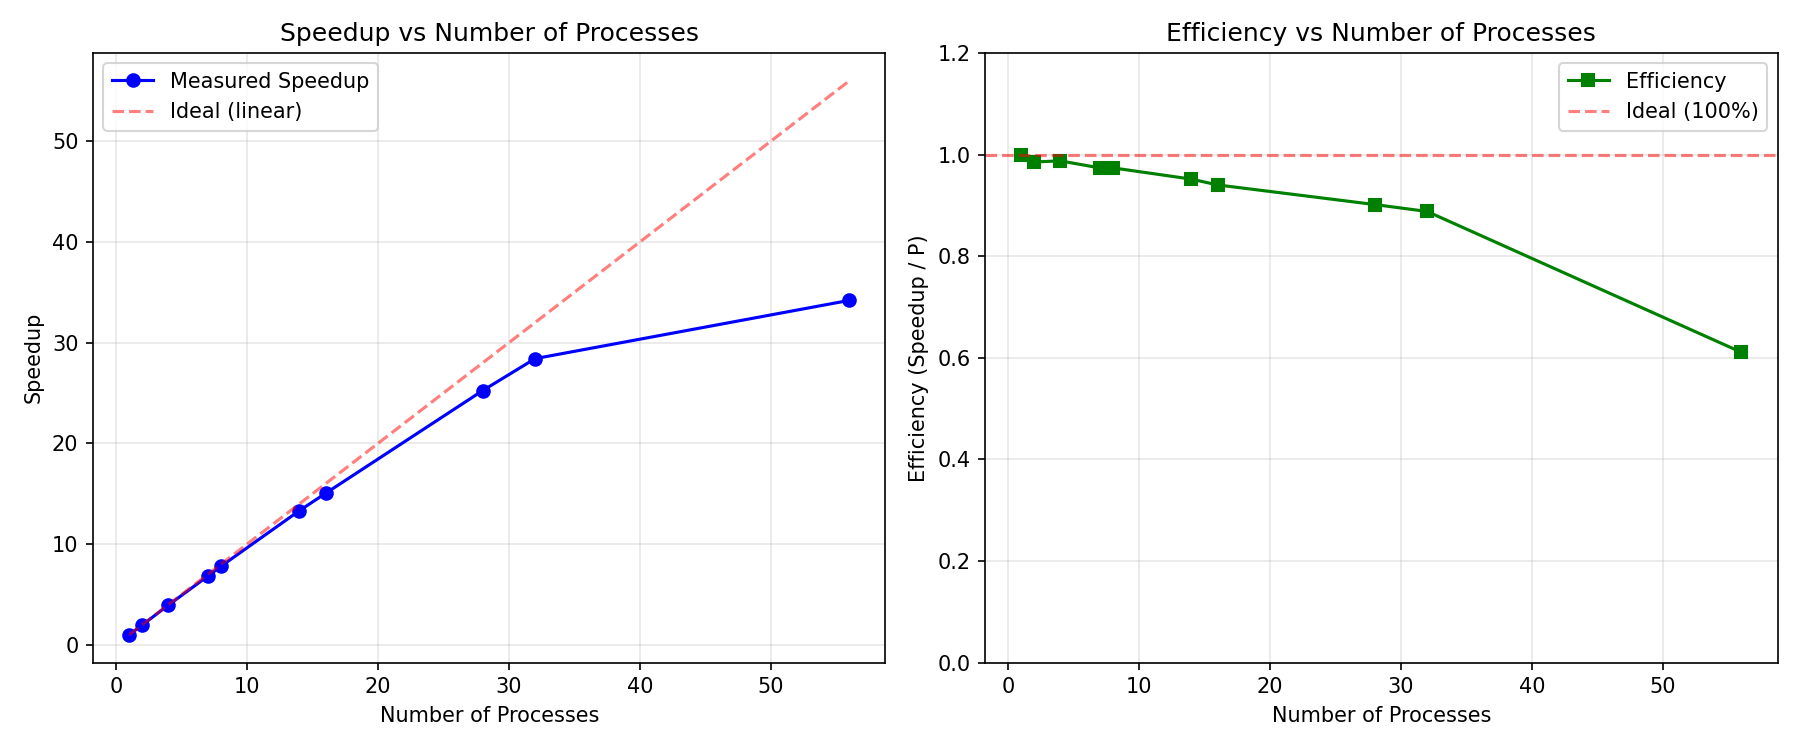
\includegraphics[width=0.95\textwidth]{speedup_efficiency.png}
\caption{Speedup (left) and efficiency (right) for the distributed gradient descent with $N = 10\,000\,000$ samples on one Toubkal node (up to 56 cores).}
\label{fig:speedup}
\end{figure}

\subsubsection{Analysis}

\begin{itemize}
    \item \textbf{Near-linear scaling up to 32 cores}: efficiency remains above 88\% ($E(32) = 0.888$), confirming that the computation-to-communication ratio is high for 10M samples.
    \item \textbf{Degradation at 56 cores}: speedup reaches $34.2\times$ but efficiency drops to 61\%. At this point each process handles only $\sim$178k samples, and the two \texttt{MPI\_Allreduce} calls per epoch become a significant fraction of the per-iteration time.
    \item \textbf{Super-linear effects}: at small core counts (2--8), efficiency is close to or slightly above the ideal, likely due to improved cache utilisation when each process operates on a smaller data subset.
    \item \textbf{Increasing $N$} shifts the crossover point to higher $P$, as confirmed by comparing with the 100k-sample run where 56-core efficiency was only 2.6\%.
\end{itemize}

% ============================================================
\section{Key Concepts Summary}

\subsection{MPI Derived Type Functions Used}

\begin{table}[H]
\centering
\begin{tabular}{@{}ll@{}}
\toprule
\textbf{Function} & \textbf{Purpose} \\
\midrule
\texttt{MPI\_Type\_vector} & Regular strided blocks (Ex.~1: column extraction) \\
\texttt{MPI\_Type\_create\_hvector} & Byte-strided replication (Ex.~1: column sweep) \\
\texttt{MPI\_Type\_create\_struct} & Heterogeneous struct layout (Ex.~2: Sample) \\
\texttt{MPI\_Type\_create\_resized} & Adjust type extent for arrays (Ex.~2) \\
\texttt{MPI\_Type\_commit} & Finalize type before use \\
\texttt{MPI\_Type\_free} & Release resources \\
\bottomrule
\end{tabular}
\end{table}

\subsection{Why Derived Types?}

\begin{itemize}
    \item \textbf{Avoid manual packing}: No need to copy data into contiguous buffers before sending.
    \item \textbf{Zero-copy transposition}: Exercise~1 transposes a matrix purely through the datatype layout --- no extra memory or loops.
    \item \textbf{Type safety}: \texttt{MPI\_Type\_create\_struct} respects struct member offsets and possible padding, ensuring portability.
    \item \textbf{Performance}: MPI implementations can optimize non-contiguous access patterns internally.
\end{itemize}

% ============================================================
\section{Conclusion}

In this practical session, we explored MPI derived datatypes through two exercises:

\begin{enumerate}
    \item \textbf{Matrix transposition} demonstrated how \texttt{MPI\_Type\_vector} and \texttt{MPI\_Type\_create\_hvector} can transform data layout during communication, achieving an in-place transposition without any additional loops or temporary buffers.
    
    \item \textbf{Distributed gradient descent} showed the practical use of \texttt{MPI\_Type\_create\_struct} for communicating complex C structures. Benchmarking on a Toubkal node with $N = 10\,000\,000$ samples demonstrated near-linear speedup up to 32 cores (efficiency $\approx 89\%$) and a $34.2\times$ speedup at 56 cores, with efficiency degrading gracefully as communication overhead grows relative to per-process computation.
\end{enumerate}

MPI derived types are a powerful abstraction that enable clean, efficient parallel code by offloading data layout transformations to the MPI runtime.

\end{document}
